\chapter[Harald's Battle]{
    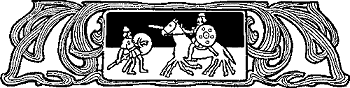
\includegraphics[width=9.3cm]{viking-tales/024}\\
    Harald's Battle}

\lettrine{N}{ow} King Halfdan had many foes. When he was alive they were
afraid to make war upon him, for he was a mighty warrior. But when Harald
became king, they said:

``He is but a lad. We will fight with him and take his land.''

So they began to make ready. King Harald heard of this and he laughed
and said:

``Good! `Foes'-fear' is thirsty, and my legs are stiff with much
sitting.''

He called three men to him. To one he gave an arrow, saying:

``Run and carry this arrow north. Give it into the hands of the master
of the next farm, and say that all men are to meet here within two weeks
from this day. They must come ready for war and mounted on horses. Say
also that if a man does not obey this call, or if he receives this arrow
and does not carry it on to his next neighbor, he shall be outlawed from
this country, and his land shall be taken from him.''

He gave arrows to the other two men and told them to run south and east
with the same message.

So all through King Harald's country men were soon busy mending helmets
and polishing swords and making shields. There was blazing of forges and
clanging of anvils all through the land.

On the day set, the fields about King Harald's house were full of men
and horses. After breakfast a horn blew. Every man snatched his weapons
and jumped upon his horse. Men of the same neighborhood stood together,
and their chief led them. They waited for the starting horn. This did
not look like our army. There were no uniforms. Some men wore helmets,
some did not. Some wore coats of mail, but others wore only their
jackets and tights of bright-colored wool. But at each man's left side
hung a great shield. Over his right shoulder went his sword-belt and
held his long sword under his left hand. Above most men's heads shone
the points of their tall spears. Some men carried axes in their belts.
Some carried bows and arrows. Many had ram's horns hanging from their
necks.

King Harald rode at the front of his army with his standard-bearer
beside him. Chain-armor covered the king's body. A red cloak was thrown
over his shoulders. On his head was a gold helmet with a dragon standing
up from it. He carried a round shield on his left arm. The king had made
that shield himself. It was of brass. The rivets were of silver, with
strangely shaped heads. On the back of Harald's horse was a red cloth
trimmed with the fur of ermine.

King Harald looked up at his standard and laughed aloud.

``Oh, War-lover,'' he cried, ``you and I ride out on a gay journey.''

A horn blew again and the army started. The men shouted as they went,
and blew their ram's horns.

``Now we shall taste something better than even King Harald's ale,''
shouted one.

Another rose in his stirrups and sniffed the air.

``Ah! I smell a battle,'' he cried. ``It is sweeter than those strange
waters of Arabia.''

So the army went merrily through the land. They carried no tents, they
had no provision wagons.

``The sky is a good enough tent for a soldier,'' said the Norsemen.
``Why carry provisions when they lie in the farms beside you?''

After two days King Harald saw another army on the hills.

``Thorstein,'' he shouted, ``up with the white shield and go tell King
Haki to choose his battle-field. We will wait but an hour. I am eager
for the frolic.''

So Thorstein raised a white shield on his spear as a sign that he came
on an errand of peace. He rode near King Haki, but he could not wait
until he came close before he shouted out his message and then turned
and rode back.

``Tell your boy king that we will not hang back,'' Haki called after
Thorstein.

King Harald's men waited on the hillside and watched the other army
across the valley. They saw King Haki point and saw twenty men ride off
as he pointed. They stopped in a patch of hazel and hewed with their
axes.

``They are getting the hazels,'' said Thorstein.

``Audun,'' said King Harald to a man near him, ``stay close to my
standard all day. You must see the best of the fight. I want to hear a
song about it after it is over.''

This Audun was the skald who sang at the drinking of King Halfdan's
funeral ale.

King Haki's men rode down into the valley. They drove down stakes all
about a great field. They tied the hazel twigs to the stakes in a
string. But they left an open space toward King Harald's army and one
toward King Haki's. Then a man raised a white shield and galloped toward
King Harald.

``We are ready!'' he shouted.

At the same time King Haki raised a red shield. King Harald's men put
their shields before their mouths and shouted into them. It made a great
roaring war-cry.

``Up with the war shield!'' shouted King Harald. ``Horns blow!''

There was a blowing of horns on both sides. The two armies galloped down
into the field and ran together. The fight had begun.

All that day long swords were flashing, spears flying, men shouting, men
falling from their horses, swords clashing against shields.

``Victory flashes from that dragon,'' Harald's men said, pointing to the
king's helmet. ``No one stands before it.''

And, surely, before night came, King Haki fell dead under
``Foes'-fear.'' When he fell, a great shout went up from his warriors,
and they turned and fled. King Harald's men chased them far, but during
the night came back to camp. Many brought swords and helmets and
bracelets or silver-trimmed saddles and bridles with them.

``Here is what we got from the foe,'' they said.

The next morning King Harald spoke to his men:

``Let us go about and find our dead.''

\begin{figure}[ht]
    \centering
    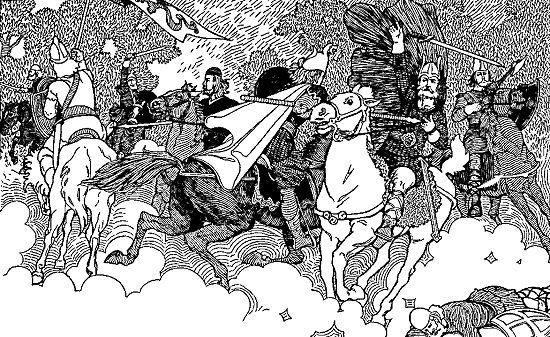
\includegraphics[width=14.6cm]{viking-tales/025}
    \caption{``King Haki fell dead under `Foes'-fear'\,''}
\end{figure}

So they went over all the battle-field. They put every man on his shield
and carried him and laid him on a hill-top. They hung his sword over his
shoulder and laid his spear by his side. So they laid all the dead
together there on the hill-top. Then King Harald said, looking about:

``This is a good place to lie. It looks far over the country. The sound
of the sea reaches it. The wind sweeps here. It is a good grave for
Norsemen and Vikings. But it is a long road and a rough road to Valhalla
that these men must travel. Let the nearest kinsman of each man come and
tie on his hell-shoes. Tie them fast, for they will need them much on
that hard road.''

So friends tied shoes on the dead men's feet. Then King Harald said:

``Now let us make the mound.''

Every man set to work with what tools he had and heaped earth over the
dead until a great mound stood up. They piled stones on the top. On one
of these stones King Harald made runes telling how these men had died.

After that was done King Harald said:

``Now set up the pole, Thorstein. Let every man bring to that pole all
that he took from the foe.''

So they did, and there was a great hill of things around it. Harald
divided it into piles.

``This pile we will give to Thor in thanks for the victory,'' he said.
``This pile is mine because I am king. Here are the piles for the
chiefs, and these things go to the other men of the army.''

So every man went away from that battle richer than he was before, and
Thor looked down from Valhalla upon his full temple and was pleased.

The next morning King Harald led his army back. But on the way he met
other foes and had many battles and did not lose one. The kings either
died in battle or ran away, and Harald had their lands.

``He has kept his vow,'' men said, ``and ground his father's foes under
his heel.''

So King Harald sat in peace for a while.
